\chapter{Antecedentes}

\section{Control de flujo de información}
Los lenguajes con tipado de seguridad para el control del flujo de la información clasifican los valores de un programa con respecto a sus niveles de confidencialidad, expresado mediante una \emph{lattice}\footnote{Un orden parcial, donde todo par de elementos tiene un único supremo e ínfimo} de etiquetas de seguridad. Por ejemplo, con la lattice de dos niveles de seguridad \texttt{L} $\sqsubseteq$ \texttt{H} se puede distinguir entre valores públicos o de baja confidencialidad (\texttt{L}) y valores privados o de alta confidencialidad (\texttt{H}). Un sistema de tipos con control de flujo asegura de forma estática el cumplimiento de la propiedad \emph{noninterference}~\cite{noninterference}, esto es, que la información confidencial no fluya directa o indirectamente hacia canales públicos~\cite{volpanoAl:S96}.

En el siguiente ejemplo se muestra un código anotado con niveles de seguridad, en donde el parámetro \texttt{guess} y el retorno del método se declaran de baja confidencialidad, y el parámetro \texttt{password} se declara de alta confidencialidad.

\begin{ej} \ \\
  \normalfont
  \label{ej2-1}
\begin{lstlisting}
  String@L login(String@L guess, String@H password) {
    if (password == guess) return "Login successful";
    else return "Login failed";
  }
\end{lstlisting}
\end{ej}

Se dice que ocurrió un \emph{flujo implícito} cuando un programa da conocimiento de una variable de baja confidencialidad, en un contexto de alta confidencialidad. En el ejemplo \ref{ej2-1}, se da conocimiento de un literal\footnote{Un literal es considerado de baja confidencialidad} en un contexto determinado por la operación de comparación del condicional, la cual retorna un valor de alta confidencialidad.

La ocurrencia de un flujo implícito significa una infracción a noninterference. Para su detección, se utiliza el concepto de \textit{program counter} (PC) para seguridad~\cite{pc}, el cual permite considerar el contexto de ejecución de una instrucción en las reglas del sistema de tipos. En el ejemplo \ref{ej2-1}, las instrucciones de retorno se ejecutan con un PC igual al nivel de seguridad de retorno de la condición.

A pesar de que noninterference es una propiedad atractiva para la especificación de sistemas seguros, se considera muy estricta en la práctica, debido a que impide que la información confidencial tenga cualquier tipo de influencia en una salida observable de un programa. En efecto, queremos que el programa de \texttt{login} sea aceptado a pesar de infringir noninterference, pues de otra forma no tendríamos cómo realizar la autenticación.

Para solucionar este problema, los lenguajes de seguridad adicionan mecanismos para disminuir el nivel de seguridad de un valor confidencial, implementados de diferentes formas~\cite{sabelfeldSands:JCS09}. Una de ellas, por ejemplo en Jif~\cite{jif} es usar un operador \texttt{declassify}, que \emph{desclasifica} un valor de alta confidencialidad retornando un valor de baja confidencialidad. En el siguiente ejemplo, se utiliza para desclasificar el resultado de la operación de comparación:

\begin{ej} \ \\
  \normalfont
  \label{ej2-2}
\begin{lstlisting}
  String@L login(String@L guess, String@H password) {
    if (declassify(password == guess)) return "Login Successful";
    else return "Login failed";
  }
\end{lstlisting}
\end{ej}



Esto no corresponde a una amenaza de seguridad, debido a que el resultado de la operación de comparación es negligible con respecto al parámetro privado \texttt{password}. Sin embargo, usos arbitrarios del operador \texttt{declassify} pueden resultar en serias fugas de información. Por ejemplo, \texttt{declassify(password)} da conocimiento absoluto sobre el valor de la variable a un observador público.

Varios mecanismos se han explorado para controlar el uso de desclasificación, y poder asegurar además una propiedad de seguridad para el programa~\cite{sabelfeldSands:JCS09}. En esta dirección, Cruz et al.~\cite{cruzAl:ecoop2017} recientemente propusieron \emph{type-based declassification} como un mecanismo de desclasificación que conecta la abstracción de tipos con una forma controlada de desclasificación, en una manera intuitiva y expresiva, proveyendo garantías formales sobre la seguridad del programa.

En type-based declassification los tipos tienen dos facetas; la faceta privada, que refleja el tipo de implementación, y la faceta pública, que refleja las operaciones de desclasificación sobre los valores de dicho tipo. Por ejemplo, el tipo $\mathtt{StringEq} \triangleq [\mathtt{eq} : \mathtt{String} \rightarrow \mathtt{Bool}]$ autoriza la operación \texttt{eq} sobre un \texttt{String}. Entonces se puede usar el tipo de dos facetas $\mathtt{String} < \mathtt{StringEq}$, en donde \texttt{String} es un subtipo de \texttt{StringEq}, para controlar la operación de desclasificación de la igualdad sobre \texttt{password}.

\begin{ej} \ \\
  \normalfont
  \label{ej2-3}
\begin{lstlisting}
  String<String login(String<String guess, String<StringEq password) {
  	if (password.eq(guess)) return "Login successful";
  	else return "Login failed";
  }
\end{lstlisting}
\end{ej}

Las facetas de desclasificación son parte de la jerarquía de tipos, por lo que forman una lattice como se muestra en la figura \ref{latticeTBD}, donde \texttt{StringEq} $\triangleq [\mathtt{eq} : \mathtt{String} \rightarrow \mathtt{Bool}]$ y \texttt{StringEqLength} $\triangleq [\mathtt{eq} : \mathtt{String} \rightarrow \mathtt{Bool}, \mathtt{length} : \mathtt{Unit} \rightarrow \mathtt{Int}]$.

	\begin{figure}[ht]
		\centering
		\begin{tikzpicture}[node distance=2.3cm]
			\node(Top) 												{\texttt{Top}};
			\node(StringEq)		[below right of=Top]			{\texttt{StringEq}};
			\node(StringEqLength)      [below of=StringEq]       {\texttt{StringEqLength}};
			\node(String)				[below of=StringEqLength]       {\texttt{String}};
			\node(int)					[below left of=Top] 			{\texttt{int}};
			\draw(Top)      -- (StringEq);
			\draw(Top)      -- (int);
			\draw(StringEq)      -- (StringEqLength);
			\draw(StringEqLength)      -- (String);
		\end{tikzpicture}
    \label{latticeTBD}
		\caption{lattice de subtyping}
	\end{figure}

Si la faceta pública coincide con la faceta privada, toda operación sobre el valor estará autorizada. Cuando esto sucede, se refiere usualmente a la faceta pública con \texttt{Bot}, por encontrarse siempre en la parte inferior de la lattice. Cuando se quiere referir a una faceta pública vacía o que no autoriza ninguna operación, se usa \texttt{Top}, por encontrarse en la parte superior de la lattice.

En estricto rigor, los métodos declarados en la faceta pública también poseen tipos de dos facetas en sus firmas. Así, el tipo StringEq visto anteriormente se define como $\mathtt{StringEq} \triangleq [\mathtt{eq} : \mathtt{String<String} \rightarrow \mathtt{Bool<Bool}]$.

Existen dos reglas principales para comprobar que un programa con facetas de desclasificación se encuentra bien tipado. En primer lugar, la llamada a un método sobre un valor cuya faceta pública autoriza la operación, retorna un valor del tipo declarado como retorno para aquella operación en la faceta pública. Por ejemplo, si tenemos un valor con faceta pública $\mathtt{StringHashEq} \triangleq [\mathtt{hash} : \mathtt{Unit<Unit} \rightarrow \mathtt{String<StringEq}]$, y llamamos al método $\mathtt{hash}$ sobre este valor, el tipo de retorno de esa llamada será $\mathtt{String<StringEq}$. A esta regla se le llama \texttt{TmD}.

La segunda regla expresa que la llamada a un método sobre un valor cuya faceta pública no autoriza la operación, retorna un valor con faceta pública \texttt{Top}. Esto ocurre, por ejemplo, si llamamos al método $\mathtt{hash}$ sobre un valor que declara la faceta pública $\mathtt{StringEq}$. A esta regla se le llama \texttt{TmH}.

La propiedad de seguridad que se demuestra para el sistema de tipos de type-based declassification es una forma de noninterference con políticas de desclasificación, denominada \emph{Relaxed noninterference}. Un lenguaje de seguridad que cumple esta propiedad, garantiza que la información confidencial sólo puede fluir hacia canales públicos de forma controlada, por medio de las políticas de desclasificación.

\section{Inferencia de tipos} \label{inference}
La inferencia de tipos es el proceso de determinar los tipos para las expresiones de un programa, basado en cómo son usadas. Tener un mecanismo de inferencia en un lenguaje de programación puede ser muy útil, debido a que da la posibilidad al programador de omitir las declaraciones de tipo para algunos identificadores.

Consideremos el siguiente ejemplo, donde se quita la anotación de la faceta pública del parámetro \texttt{password} del ejemplo \ref{ej2-3}:

\begin{ej} \ \\
  \normalfont
  \label{ej2-4}
\begin{lstlisting}
  String<String login(String<String guess, String password) {
  	if (password.eq(guess)) return "Login successful";
  	else return "Login failed";
  }
\end{lstlisting}
\end{ej}

Basado en el uso del parámetro \texttt{password}, el sistema de tipos podría \emph{inferir} que su faceta pública contiene al menos el método \texttt{eq}.

Para razonar acerca de expresiones con tipos desconocidos, los lenguajes de programación incluyen \emph{variables de tipo} en sus sistemas de tipos. En el ejemplo \ref{ej2-4}, se asigna un tipo $\mathtt{\alpha}$ a la faceta pública del parámetro \texttt{password}.

\subsection{Constraints} \label{constraints}
Cuando un sistema de tipos aplica una determinada regla para tipar una expresión, puede imponer condiciones que los tipos deben cumplir para que la expresión esté bien tipada. En el ejemplo \ref{ej2-4}, se puede decir que \texttt{password} tiene una faceta pública $\mathtt{\alpha}$ si y solo si $\mathtt{\alpha}$ posee el método \texttt{eq}.

Para razonar acerca de estas condiciones, el sistema de tipos las representa mediante \emph{constraints}, que expresan una relación entre dos tipos. En el ejemplo \ref{ej2-4}, la condición sobre la faceta pública de \texttt{password} puede ser representada mediante la constraint de subtyping $\{\alpha <: [\mathtt{eq} : \mathtt{String<String} \rightarrow \mathtt{Bool<Bool}]\}$.

El uso de constraints permite la presentación de un algoritmo de inferencia de forma modular, como un generador de constraints y un solucionador de constraints. El \emph{set de constraints} generado se asemeja a un sistema de ecuaciones que siempre tendrá solución dependiendo de las características del lenguaje de programación. Por ejemplo, System F~\cite{WELLS1999111} es un lenguaje con inferencia de tipos completa no decidible.

\subsection{Unificación}
La unificación es el proceso de encontrar una solución a las variables de tipo del set de constraints. Si las constraints son de igualdad, la unificación realiza substituciones sucesivas hasta resolver cada uno de los tipos. En cambio, si las constraints son de subtyping, se deben realizar las operaciones \texttt{meet} (el ínfimo entre dos elementos, $a \wedge b$) y \texttt{join} (el supremo entre dos elementos, $a \vee b$) sobre la lattice que conforma la jerarquía de tipos, cuando sea pertinente.

\begin{figure}[ht]
  \centering
  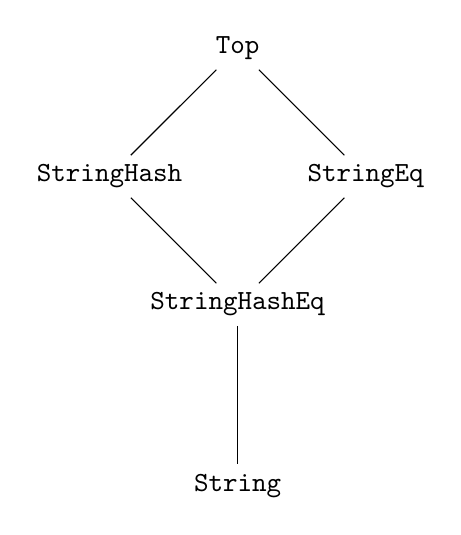
\begin{tikzpicture}[node distance=2.3cm]
    \node(Top) 												{\texttt{Top}};
    \node(StringEq)		[below right of=Top]			{\texttt{StringEq}};
    \node(StringHash)					[below left of=Top] 			{\texttt{StringHash}};
    \node(StringHashEq) [below left of=StringEq] {\texttt{StringHashEq}};
    \node(String) [below of=StringHashEq] {\texttt{String}};
    \draw(Top)      -- (StringEq);
    \draw(Top)      -- (StringHash);
    \draw(StringEq)      -- (StringHashEq);
    \draw(StringHash)      -- (StringHashEq);
    \draw(StringHashEq) -- (String);
  \end{tikzpicture}
  \caption{Operación \texttt{meet} entre \texttt{StringEq} y \texttt{StringHash}}
  \label{latticeInference}
\end{figure}

Consideremos el siguiente ejemplo, en donde se modifica una expresión de retorno del ejemplo \ref{ej2-4} con otro uso del parámetro \texttt{password}.

\begin{ej} \ \\
  \normalfont
  \label{ej2-5}
\begin{lstlisting}
  String<String login(String<String guess, String password) {
  	if (password.eq(guess)) return password.hash();
  	else return "Login failed";
  }
\end{lstlisting}
\end{ej}

Supongamos que \texttt{hash} retorna un \texttt{String}. Ahora se generan dos constraints sobre \texttt{password}, $\{\alpha <: [\mathtt{eq} : \mathtt{String<String} \rightarrow \mathtt{Bool<Bool}]\}$ y $\{\alpha <: [\mathtt{hash} : \mathtt{Unit<Unit} \rightarrow \mathtt{Bool<Bool}]\}$. El tipo $\alpha$ se resuelve con la operación \texttt{meet} entre ambos tipos de objeto, cuyo resultado $\mathtt{StringHashEq} \triangleq [\mathtt{eq} : \mathtt{String<String} \rightarrow \mathtt{Bool<Bool}, \mathtt{hash} : \mathtt{Unit<Unit} \rightarrow \mathtt{Bool<Bool}]\}$ se muestra en la figura \ref{latticeInference}.

En general, se aplican las siguientes reglas para la aplicación de las operaciones sobre la lattice:

\begin{teo} \label{teo1} \normalfont Si \texttt{x}, \texttt{y} y \texttt{z} pertenecen a una lattice de subtyping, se cumple lo siguiente: \\
  \begin{itemize}
    \item \texttt{x <: y}, \texttt{x <: z} $\implies$ \texttt{x <: y }$\wedge$\texttt{ z}
    \item \texttt{y <: x}, \texttt{z <: x} $\implies$ \texttt{y }$\vee$\texttt{ z <: x}
  \end{itemize}
\end{teo}
